\documentclass[11pt]{article}

\usepackage[margin=1in]{geometry}
\usepackage[utf8]{inputenc}
\usepackage[T1]{fontenc}
\usepackage{newtxtext,newtxmath}
\usepackage[numbers,sort&compress]{natbib}
\usepackage{xcolor}
\usepackage[colorlinks=true,linkcolor=blue!60!black,citecolor=blue!60!black,urlcolor=blue!60!black]{hyperref}
\usepackage{url}
\usepackage{booktabs}
\usepackage{amsfonts}
\usepackage{nicefrac}
\usepackage{microtype}
\usepackage{graphicx}
\usepackage{multirow}
\usepackage[section]{placeins}  % keep floats inside their own section
\setlength{\emergencystretch}{2em}  % avoid overfull lines from long words and code names

% Placeholder for unfinished results. scripts/check_paper.sh fails the build if any remain.
\newcommand{\pending}[1]{\textcolor{red}{\textbf{[PENDING: #1]}}}

\title{Trial Order, Recording Time, and Checkpoint Selection\\in a 39-Way Imagined-Speech EEG Benchmark}
\author{Noel Sason\\
  University of California, Berkeley\\
  \texttt{noel\_sason@berkeley.edu}}
\date{October 2026}

\begin{document}
\maketitle

\begin{abstract}
Imagined-speech EEG classifiers report small margins above chance, so the evaluation protocol decides
what those margins mean. We audit the 39-way semantic-category benchmark released with Chisco, a
large public imagined-speech corpus, for participant S1, using the released code. Its stimulus
order is clustered by category, and its split places each evaluation trial between two training
trials, almost always from the same recording run. A classifier that never sees EEG and copies the label of the preceding
training trial scores 18.8\% on the released evaluation set, above the published 13.88\%, and
per-trial EEG summary statistics identify a held-out trial's recording run with 98.8\% accuracy.
Running the released script with its documented configuration on our hardware prints 9.69\%. Its
reporting rule, the best of several hundred evaluations on the evaluation set, gives 6.4\% to a model
trained on permuted labels. When whole runs are held out, real labels beat permuted labels by 0.64
points, within the variation between seeds, and a reading-task control shows that the pipeline has
limited sensitivity once recording-time cues are gone. The published number therefore does not, on its
own, establish semantic decoding. We recommend reporting position-only baselines on the exact split,
holding out whole runs, and selecting checkpoints on data that is never scored. Code, tests and
result files are available at \url{https://github.com/NoelSason/eegwords}.
\end{abstract}

\section{Introduction}
\label{sec:intro}

A system that could recover the meaning of silently imagined speech from scalp EEG would be useful
to people who cannot speak, and it would be cheap and non-invasive. Reported accuracies for this
task are low, so small differences carry the argument: a result of 14\% on a 39-way problem is
interesting only if one is confident that the 11 points above chance come from the imagined
sentence and not from something else the recording happens to encode.

EEG makes that confidence hard to earn. Recordings are long, and EEG contains temporal
correlations that make trials recorded close together resemble each other regardless of the
stimulus; a classifier can exploit them by learning \emph{when} a trial was recorded
\citep{li2021perils}. Whether that matters depends on
two design choices that are easy to make and easy to overlook: the order in which stimuli are
presented, and how test trials are drawn from the recording.

We examine one benchmark where both choices interact with a third, the rule used to report
accuracy. Chisco \citep{zhang2024chisco} is a large public imagined-speech corpus: over 6{,}000
sentences per participant, recorded across five days and labelled with 39 semantic categories.
Its authors report 13.88\% category accuracy for participant S1 against a 5.52\% shuffled-label
baseline, and conclude that the EEG contains semantic information. The released code assigns every
fifth trial in recording order to the evaluation set and reports the best evaluation accuracy seen
during training.

Our central observation needs no EEG. In the released recording order, consecutive trials share a
category 19.7\% of the time, against 2.95\% if the same categories were shuffled. On the released
evaluation set, a classifier that copies the label of the preceding training trial scores
\textbf{18.8\%}, above the published EEG result. The EEG, in turn, carries the time stamp this
classifier needs: per-trial channel means and variances identify the recording run of a held-out
trial with 98.8\% accuracy. Running the released script with its documented command on our
hardware prints 9.69\%, not 13.88\%. Under the same rule, a model trained on permuted labels still
reports 6.4\%, and real labels add 2.4 points to that, not the 8.4 the paper reports. When whole
runs are held out so that evaluation trials have no neighbours in the training set, the margin
between real and permuted labels falls to 0.64 points, within the variation between seeds.

Our contributions are:
\begin{itemize}
\item An audit of the released 39-way benchmark on its exact evaluation split: trial position alone
predicts the category better than the published EEG model, and content-free EEG summary statistics
carry enough recording-time information to exploit that structure (Section~\ref{sec:audit}).
\item A re-run of the published configuration, including the released script itself, that reads
three selection rules from the same training runs and compares each with a permuted-label null
(Section~\ref{sec:results}). The published best-checkpoint rule adds 1.4--1.6 points over a
validation-selected checkpoint and reports 5.2--6.4\% for models trained without label information.
\item A split comparison showing the real-vs-permuted margin shrinking from 2.11 points on the
released split to 0.64 under run holdout (Section~\ref{sec:splits}).
\item A short protocol for temporally ordered decoding benchmarks: report a position-only baseline
on the exact evaluation split, hold out whole runs or sessions, select checkpoints on data that is
never scored, and compare against a permuted-label null run through the same pipeline.
\end{itemize}

We do not claim that the Chisco EEG contains no semantic information, or that imagined-speech
decoding from EEG is infeasible. Our claims are about what this benchmark's protocol can and
cannot show, for one participant.

\section{Related work}
\label{sec:related}

\paragraph{Imagined-speech EEG.}
\citet{panachakel2021} review a decade of systems that decode covert or imagined speech from EEG
and note that differences in acquisition and algorithms make implementations hard to compare.
Chisco \citep{zhang2024chisco} is, by its authors' account, the largest per-participant corpus for
decoding neural language: more than 6{,}000 everyday Chinese sentences per participant, recorded over five days with a 128-channel cap,
labelled with 39 semantic categories. Its Technical Validation reports 39-way category accuracies of
13.59--14.02\% for three participants, against shuffled-label baselines of 5.52--5.93\%, using an
EEGNet front end \citep{lawhern2018} followed by a Transformer encoder \citep{vaswani2017}.

\paragraph{Temporal confounds in EEG classification.}
\citet{li2021perils} showed that published results on an EEG image-classification dataset depend on
a block design, in which all stimuli of a class are presented together, and fail with a rapid-event
design in which classes are randomly intermixed: classifiers learned block-level temporal
correlations present in all EEG data, and every test trial shared a block with many training
trials. \citet{roy2019} reviewed 154 deep-learning EEG studies and recorded, for each, how
reproducible its experiments were. A concurrent public code release
\citep{concurrentaudit} audits sentence-level decoding on Chisco and a second corpus for run-identity
and stimulus-order confounds. We did not find an accompanying paper; we cite it as software and do
not claim its findings. Our audit targets the 39-way category benchmark as released, and the
reporting rule of the released code.

\paragraph{Leakage and selection bias.}
\citet{kapoor2023leakage} survey leakage in 294 papers across 17 fields that adopted ML and
propose a taxonomy of eight leakage types. Selecting a model on the same data used to estimate its performance biases that estimate upward
\citep{cawley2010}, and with small test sets the variance of a single accuracy estimate is itself
large \citep{varoquaux2018}. The released Chisco code combines both: test trials are neighbours of
training trials, and the reported figure is the best of 313 evaluations on that same set (Section~\ref{sec:setting}).

\section{Experimental setting}
\label{sec:setting}

\paragraph{Data.}
We use participant S1 (\texttt{sub-01}) of Chisco \citep{zhang2024chisco}, distributed as OpenNeuro
\texttt{ds005170} \citep{ds005170}. In each trial the participant reads and memorises a sentence (the first 5\,s), then imagines
saying it (the next 3.3\,s). The paper reports 6{,}681 presented sentences per
participant over five recording days. The released preprocessed imagined-speech epochs for S1
contain 6{,}243 of them: within each of the 45 runs, the released trials are an in-order subsequence
of that run's stimulus list, so preprocessing removed 438 trials and reordered none. Each epoch has
125 channels at 500\,Hz (1{,}651 samples); as in the released code we keep the 122 EEG channels and
scale volts to microvolts, with no further normalisation. Every sentence maps to one of 39 semantic
categories through the released \texttt{textmaps.json}. Uniform chance is $1/39 = 2.56\%$; always
predicting the most frequent training category scores 4.72\% on the evaluation set described below.

\paragraph{The published protocol, as released.}
The paper describes the model (an EEGNet front end, one Transformer encoder layer, mean pooling,
a linear classifier) but not the split, the number of training runs, or how the reported accuracy is
chosen. We take these from the released code \citep{chiscocode} and the command its README gives
for ``reproducing the paper results'' (Appendix~\ref{app:upstream}). Trials from all 45 runs are
concatenated in recording order and every trial whose position satisfies $i \bmod 5 = 1$ is placed in
the evaluation set (1{,}249 trials); the other 4{,}994 are used for training. There is no third set.
Training runs for 100 epochs with AdamW (learning rate $5\times10^{-4}$, weight decay 0.01, batch 16,
linear warm-up over the first 10\% of steps, then linear decay). Every 100 optimiser steps the model
is evaluated on the evaluation set, and the script prints the maximum accuracy seen over all
evaluations: 313 of them in this configuration. We call this the \emph{max-over-checkpoints} rule.
Table~3 of the paper reports 13.88\% for S1 and a 5.52\% baseline obtained by shuffling the
correspondence between EEG and labels in training.

\paragraph{Our re-implementation.}
We copy the released model code and change only how its two temporal convolutions are computed
(an equivalent unfold-and-multiply form with the same parameters and initialisation, which is
about nine times faster on our hardware; outputs agree with the original to float32 rounding).
Data loading, label mapping and the split follow the released code and are checked by unit tests.
To read a second selection rule from the same runs, we hold out a random 10\% of the training
trials (499) as a validation set, so our models train on 4{,}495 trials and are evaluated
281 times. All runs use Apple-silicon GPUs (PyTorch MPS, float32) and three seeds.

\paragraph{Three readings of one run.}
For every run we store validation and evaluation-set accuracy at every evaluation, and the
evaluation-set predictions at three checkpoints:
\textbf{max-over-checkpoints} (the published rule);
\textbf{validation-selected}, the checkpoint with the highest validation accuracy, scored once on
the evaluation set, which is never used for selection; and
\textbf{last}, the final checkpoint.
Because all three come from the same training run, differences between them are due to the
selection rule alone.

\paragraph{Splits.}
Besides the released split (\emph{interleaved}) we use three others, each leaving about 80\% of
trials for training:
\emph{random-trial} (a random 20\% of trials);
\emph{run holdout} (the 45 runs in five fixed folds of nine runs; we report held-out folds 0--2); and
\emph{session holdout} (one recording day held out at a time; we report days 1--3).
For the grouped splits the validation set is made of whole training runs, so model selection is also
free of within-run neighbours. For cost reasons the split comparison uses the same model at
250\,Hz (pairwise averaging) and 30 epochs; it is compared only within itself. As a positive control
we also train on the reading epochs (the first 5\,s of each trial; 6{,}387 released epochs for S1,
2{,}501 samples at 500\,Hz), whose labels and trial order follow the same stimulus lists.

\paragraph{Permutation control.}
For each configuration we also train with the training labels randomly permuted; validation and
evaluation labels are untouched. This mirrors the shuffled baseline in the released code and gives
the accuracy each selection rule produces when the EEG carries no information about the label.

\paragraph{Uncertainty.}
The unit of replication for EEG models is a training seed ($n=3$). We report per-seed values, means
and standard deviations, and do not run significance tests on three seeds. For accuracies of a single
classifier on the evaluation set we report 95\% intervals from a bootstrap that resamples test
\emph{runs} (2{,}000 draws), because trials within a run share stimulus-list structure and are not
independent.

\section{Auditing the evaluation set without EEG}
\label{sec:audit}

\paragraph{The stimulus order is clustered by category.}
In the released trial order, 19.7\% of consecutive trials share a category. If the same category
frequencies were in random order, 2.95\% would. The excess decays with distance but persists: 14.2\%
at lag 2, 8.9\% at lag 5, 6.7\% at lag 10 and 5.2\% at lag 50 (Figure~\ref{fig:order}). Restricting
to pairs within the same run changes these by at most 0.6 points. Runs are also unevenly composed:
a run contains a median of 30 of the 39 categories, and its most frequent category makes up a median
12.9\% of its trials (maximum 33.6\%). The trial's position within its run carries no category
information: predicting the most common training category at the same position across runs scores
3.7\%, below the majority-class rate.

\begin{figure}[t]
  \centering
  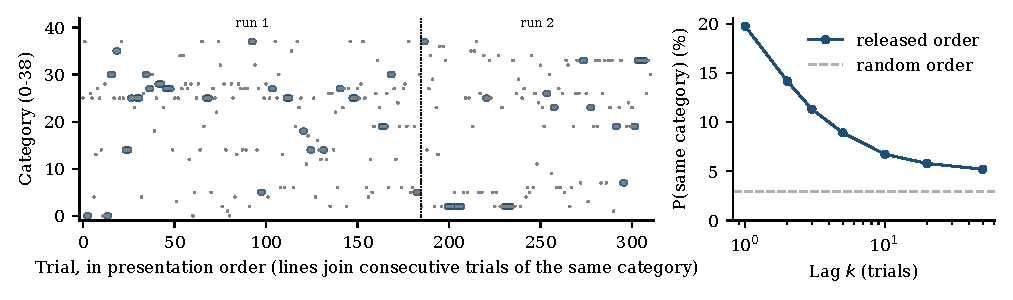
\includegraphics[width=\linewidth]{figures/fig_order.pdf}
  \caption{\textbf{Category order in the released S1 recording.} Left: category of each trial in
  runs 1--3, in presentation order (white lines separate runs). Right: probability that two trials
  $k$ positions apart share a category, against the value expected if the same categories were
  presented in random order (dashed). Source: \texttt{results/label\_baselines.json}.}
  \label{fig:order}
\end{figure}

\paragraph{Classifiers that never see EEG.}
On the released split, every evaluation trial sits between two training trials. We evaluate
classifiers that use only the training labels and each evaluation trial's position in the recording
(Table~\ref{tab:noeeg}). Copying the label of the nearest earlier training trial scores
\textbf{18.82\%} (95\% CI 16.49--21.57) on the published evaluation set, above the 13.88\% the paper
reports with EEG. A five-nearest-neighbour vote over trial position scores 20.90\%, and knowing only
which run a trial came from (predicting that run's most common training category) scores 14.41\%.
These classifiers are fitted on training labels only; none of them reads an evaluation label.

Two order controls locate the information. Shuffling all labels across the recording (1{,}000
permutations) drops the copy-previous classifier to 2.92\% on average (maximum 4.24\%). Shuffling
labels only within each run, which keeps each run's category mix but destroys the order inside it,
drops it to 5.96\% (maximum 8.25\%). Most of the 18.8\% therefore comes from adjacency within runs,
and a smaller part from run composition.

When whole runs are held out, the neighbouring training trial belongs to a different run and these
classifiers lose their advantage: copy-previous scores 2.42--5.67\% across the five run folds, and
the five-nearest vote 3.05--8.58\%.

\begin{table}[t]
\centering
\small
\caption{\textbf{Classifiers that never see EEG}, scored on the evaluation trials of each split (accuracy, \%). Each uses only training labels and the trial's position in the recording. Interleaved is the released split. Grouped splits: mean over the five folds, with the range in brackets. Uniform chance is 2.56\%. Source: \texttt{results/label\_baselines.json}.}
\label{tab:noeeg}
\setlength{\tabcolsep}{4pt}
\begin{tabular}{lcccc}
\toprule
Classifier & Interleaved & Random trial & Run holdout & Session holdout \\
\midrule
Majority class & 4.72 & 4.56 & 3.46 [2.64, 4.60] & 1.91 [0.59, 3.65] \\
Previous training trial & 18.82 & 18.57 & 4.28 [2.42, 5.67] & 3.40 [0.20, 6.84] \\
Next training trial & 20.42 & 18.57 & 5.47 [3.62, 7.69] & 3.67 [0.20, 7.62] \\
5 nearest training trials & 20.90 & 21.70 & 5.97 [3.05, 8.58] & 3.28 [0.20, 5.90] \\
Majority within run & 14.41 & 14.01 & 3.46 [2.64, 4.60] & 1.91 [0.59, 3.65] \\
Majority at run position & 3.68 & 3.52 & 3.48 [3.21, 3.77] & 3.09 [2.57, 3.79] \\
\bottomrule
\end{tabular}
\end{table}


\paragraph{EEG carries a recording-time signature.}
An EEG model can only use the order structure if the signal tells it when a trial was recorded.
We test this with deliberately content-poor features: the mean and log-variance of each channel over
the 3.3\,s epoch (244 numbers per trial, no waveform), fed to a multinomial logistic regression.
On the released split, these features identify which of the 45 runs a held-out trial came from with
\textbf{98.8\%} accuracy (chance 2.2\%). Trained to predict category instead, the same model scores
\textbf{9.05\%} on the published evaluation set (permuted-label null: mean 3.11\%, maximum 3.84\% over
five permutations) and 7.37\% on a random-trial split, but 3.55\% under run holdout (null 2.76\%,
maximum 3.77\%) and 3.08\% under session holdout (null 2.79\%). Per-trial summary statistics are
enough to recover two-thirds of the published accuracy, and only when evaluation trials have
training neighbours from the same run.

\section{Re-running the published configuration}
\label{sec:results}

\paragraph{The released script.}
We ran the released \texttt{EEGclassify.py} with the README command (seed 42) on our hardware
(Appendix~\ref{app:upstream}). It printed 9.69\%. This is the highest of its 313 evaluation-set
accuracies, reached in epoch 66; we checked that the printed value equals the maximum of the logged
curve. The last checkpoint scored 7.77\%, and evaluation accuracy after the 10-epoch warm-up averaged
7.40\% (SD 0.84). The published 13.88\% is 4.2 points above the best value this run reached.

\paragraph{Our re-implementation matches the released script.}
With the same configuration, the per-epoch training loss of our re-implementation differs from
that of the released script by at most 0.043 (mean 0.016) across three seeds, ending at 3.37--3.40 against
3.40, and the evaluation curves overlap (Appendix Figure~\ref{fig:upstream}). Under the published rule it scores 8.75\% $\pm$ 0.67 over three
seeds (8.33, 8.41, 9.53), against 9.69\% for the released script's single seed. Neither reaches
13.88\%. We do not know what accounts for the remaining difference; candidates include hardware,
seed, and software versions, and we could not test the authors' environment.

\paragraph{Three selection rules, real and permuted labels.}
Table~\ref{tab:repro} reads three rules from the same runs. Taking the best of 281 evaluations gives
8.75\% with real labels and 6.38\% with permuted training labels; the permuted value is 0.9 points
above the paper's own shuffled baseline (5.52\%), which used the same rule. Choosing the checkpoint on
held-out validation data instead gives 7.13\% and 5.02\%, and the last checkpoint 7.39\% and 4.80\%.
The max rule therefore adds 1.6 points to the real-label result and 1.4 to the permuted one; in both
cases the maximum sits above the average over all post-warm-up evaluations (7.01\% real, 5.02\%
permuted) by 1.75 and 1.35 points (Figure~\ref{fig:curves}). Real labels beat permuted labels by 2.1
to 2.6 points under every rule. The published margin is 8.4.

\begin{table}[t]
\centering
\small
\caption{\textbf{One configuration, three readings.} Accuracy (\%) on the released evaluation set
(1{,}249 trials) for the published configuration (500\,Hz, 100 epochs), mean $\pm$ SD over three
seeds, read from the same runs under three selection rules. Permuted: training labels shuffled,
evaluation labels intact. The 95\% CI for the no-EEG classifier is a run-clustered bootstrap.
Source: \texttt{results/summary.json}, generated by \texttt{scripts/generate\_tables.py}.}
\label{tab:repro}
\begin{tabular}{lccc}
\toprule
Selection rule & Real labels & Permuted training labels & Difference \\
\midrule
Max over checkpoints (published rule) & 8.75 $\pm$ 0.67 & 6.38 $\pm$ 0.30 & 2.38 \\
Validation-selected checkpoint & 7.13 $\pm$ 0.24 & 5.02 $\pm$ 0.76 & 2.11 \\
Last checkpoint & 7.39 $\pm$ 0.73 & 4.80 $\pm$ 0.70 & 2.59 \\
\midrule
Released script, seed 42, max over checkpoints & 9.69 & -- & -- \\
Released script, seed 42, last checkpoint & 7.77 & -- & -- \\
Published \citep[Table 3, S1]{zhang2024chisco} & 13.88 & 5.52 & 8.36 \\
\midrule
No EEG: label of previous training trial & \multicolumn{3}{l}{18.82 (95\% CI 16.49--21.57)} \\
No EEG: majority class & \multicolumn{3}{l}{4.72} \\
Uniform chance ($1/39$) & \multicolumn{3}{l}{2.56} \\
\bottomrule
\end{tabular}

\end{table}


\begin{figure}[t]
  \centering
  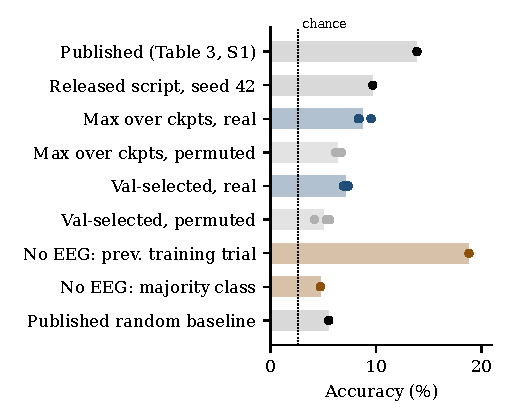
\includegraphics[width=0.49\linewidth]{figures/fig_main.pdf}\hfill
  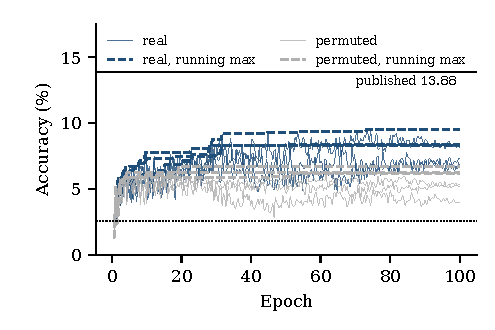
\includegraphics[width=0.49\linewidth]{figures/fig_curves.pdf}
  \caption{\textbf{Left:} accuracy on the released evaluation set. Bars are means, dots are seeds;
  ``Max over ckpts'' is the published selection rule, ``Val-selected'' the checkpoint with the best
  held-out validation accuracy; the brown bars use no EEG. \textbf{Right:} evaluation-set accuracy
  at each of the 281 evaluations of the published configuration (three seeds each), with running
  maxima (dashed); the published rule reports the end point of the dashed line.
  Source: \texttt{results/imagine\_full\_500hz\_interleaved\_*\_e100\_seed*.json}.}
  \label{fig:curves}
\end{figure}

\paragraph{Does the EEG model use the order structure?}
On the released split, the nearest earlier training trial shares the evaluation trial's category for
18.8\% of evaluation trials. At the validation-selected checkpoint, real-label models predict that
neighbour's category for 6.5--7.6\% of evaluation trials, 2.4--3.7 points more than their own class
frequencies would produce if predictions were independent of the neighbour (3.8--4.1\%).
Permuted-label models show no excess (4.1--4.6\% observed vs.\ 4.4--4.6\% expected). Real-label
accuracy is 11.8\% on trials whose neighbour shares the category and 6.0\% on the rest; for permuted
labels the corresponding values are 6.8\% and 4.6\%, so part of this gap reflects class frequency
rather than neighbour copying. The trials whose neighbour differs are not leak-free either:
predicting the most common training category of the trial's run scores 10.7\% on them without EEG.
On the released split, then, the real-label model's advantage over its null is at least partly
mediated by the recording-time structure that the no-EEG classifiers exploit. Whether any advantage
remains without that structure is the question of the next section.

\section{Changing the split}
\label{sec:splits}

We trained the same model under four splits, each with real and permuted training labels
(Table~\ref{tab:splits}, Figure~\ref{fig:splits}; 250\,Hz, 30 epochs, three seeds, three folds per
seed for grouped splits).

\paragraph{The real-vs-permuted margin shrinks as neighbours are removed.}
With the validation-selected checkpoint, real labels beat permuted labels by 2.11 points on the
released split and 1.01 on a random-trial split, both of which leave nearly every evaluation trial
with training neighbours from its own run (the position-only classifier scores 18.82\% and 18.25\% on
them). Holding out whole runs removes those neighbours: accuracy falls to 4.37\% for real labels and
3.73\% for permuted labels, a difference of 0.64 points. Paired by seed and fold, real labels are
ahead in 7 of 9 comparisons, with differences from $-2.42$ to $+2.71$ points; the mean difference is
about the size of the seed-to-seed standard deviation (0.49 real, 0.60 permuted). With three seeds
and three folds we cannot distinguish a residual signal of this size from none. Holding out a whole
recording day gives 2.55\% and 2.75\%, both at uniform chance; because the category mix differs
between days (Appendix~\ref{app:data}), we do not interpret this split further.

\paragraph{The published rule produces above-chance numbers without information.}
Under session holdout, where the validation-selected checkpoint is at chance for both conditions,
taking the best evaluation-set accuracy over training reports 5.66\% for real labels and 5.26\% for
permuted labels, more than double uniform chance. Under run holdout the same rule reports 6.27\% and
5.37\%. A best-of-many-evaluations number on the evaluation set is therefore not a reliable
indicator of decoding, even when the split itself is sound.

\begin{table}[t]
\centering
\small
\caption{\textbf{Split comparison} (accuracy, \%; 250\,Hz, 30 epochs). EEG columns: mean $\pm$ SD
over three seeds; for run and session holdout each seed's value is the mean over three held-out
folds. No-EEG columns are computed on exactly the same evaluation folds. Source:
\texttt{results/summary.json}.}
\label{tab:splits}
\setlength{\tabcolsep}{4pt}
\begin{tabular}{lccccc}
\toprule
 & \multicolumn{3}{c}{EEG model} & \multicolumn{2}{c}{No EEG} \\
\cmidrule(lr){2-4}\cmidrule(lr){5-6}
Split & Real & Permuted & Difference & Prev.\ trial & Majority \\
\midrule
\multicolumn{6}{l}{\emph{Validation-selected checkpoint}} \\
Interleaved (released) & 7.58 $\pm$ 1.04 & 5.47 $\pm$ 0.48 & 2.11 & 18.82 & 4.72 \\
Random trial & 5.79 $\pm$ 1.24 & 4.78 $\pm$ 0.53 & 1.01 & 18.25 & 4.70 \\
Run holdout & 4.37 $\pm$ 0.49 & 3.73 $\pm$ 0.60 & 0.64 & 4.02 & 3.36 \\
Session holdout & 2.55 $\pm$ 0.13 & 2.75 $\pm$ 0.43 & $-$0.20 & 3.28 & 2.58 \\
\multicolumn{6}{l}{\emph{Max over checkpoints (published rule)}} \\
Interleaved (released) & 8.17 $\pm$ 0.24 & 6.06 $\pm$ 0.18 & 2.11 &  &  \\
Random trial & 6.99 $\pm$ 0.88 & 5.20 $\pm$ 0.37 & 1.79 &  &  \\
Run holdout & 6.27 $\pm$ 0.08 & 5.37 $\pm$ 0.76 & 0.90 &  &  \\
Session holdout & 5.66 $\pm$ 1.22 & 5.26 $\pm$ 0.54 & 0.40 &  &  \\
\bottomrule
\end{tabular}

\end{table}

\begin{figure}[t]
  \centering
  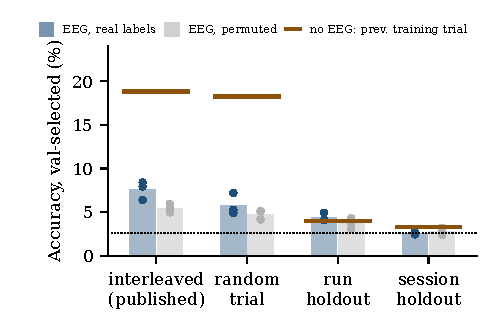
\includegraphics[width=0.62\linewidth]{figures/fig_splits.pdf}
  \caption{\textbf{Holding out whole runs.} Validation-selected accuracy by split for real (blue)
  and permuted (grey) training labels; dots are seeds. Brown lines: the position-only classifier on
  the same evaluation folds. Dotted line: uniform chance (2.56\%).}
  \label{fig:splits}
\end{figure}

\paragraph{Reading-task positive control.}
To see how much this pipeline can detect once recording-time cues are removed, we trained the same
model on the reading epochs of the same trials (Table~\ref{tab:read}). Reading is a visual task, and
we expected it to be at least as decodable as imagination. On the released split, reading scores
6.99\%, slightly below imagined speech (7.58\%). Under run holdout it scores 4.85\% against 3.75\% for
permuted labels, a difference of 1.10 points; real labels are ahead in 7 of 9 seed-fold pairs
(range $-0.46$ to $+4.34$), and most of the difference comes from one of the three held-out folds.
The pipeline therefore has limited sensitivity to category information when the order structure is
removed, for reading as well as for imagination. The small run-holdout margin for imagined speech
should be read with that in mind: it is weak evidence in either direction, not evidence of absence.

\begin{table}[t]
\centering
\small
\caption{\textbf{Reading-task control} (validation-selected accuracy, \%; 250\,Hz, 30 epochs; 6{,}387
reading epochs of 5\,s). The last column repeats the imagined-speech difference from
Table~\ref{tab:splits} for comparison. The permuted-label reading model was run only for run
holdout.}
\label{tab:read}
\begin{tabular}{lcccc}
\toprule
Task, split & Real & Permuted & Difference & Imagined: difference \\
\midrule
Reading, interleaved (released) & 6.99 $\pm$ 0.53 & not run & -- & 2.11 \\
Reading, run holdout & 4.85 $\pm$ 0.40 & 3.75 $\pm$ 0.54 & 1.10 & 0.64 \\
\bottomrule
\end{tabular}

\end{table}

\section{Discussion}
\label{sec:discussion}

\paragraph{What the results show.}
Three findings hold regardless of how the residual run-holdout margin is eventually resolved.
First, the released evaluation set can be predicted from trial position alone at 18.8\%, so an
accuracy on that split is not, by itself, evidence of decoding. Second, the released
code and configuration did not produce 13.88\% on our hardware: the released script printed 9.69\%
and our re-implementation 8.75\% $\pm$ 0.67 under the same rule. Third, the published selection rule
reports 5.2--6.4\% for models trained on permuted labels, so the paper's own shuffled baseline
(5.52\%) is the right reference for its number, and the margin over it on our runs is 2.4 points,
not 8.4. Under run holdout, where the order structure cannot help, real labels lead permuted labels
by 0.64 points, inside the seed-to-seed spread, and the reading epochs, which we expected to be
easier, reach only 1.10 points over their own null under the same split.

\paragraph{What they do not show.}
They do not show that the Chisco EEG contains no semantic information, that the published model
reached its accuracy through the order structure, or that the same holds for the other participants.
A 0.64-point margin with three seeds and three folds is compatible with a small real effect and with
none; resolving it needs more seeds, more folds and other participants, not a different reading of
these numbers. They also do not show why the published value is higher than ours.

\paragraph{Recommendations for temporally ordered decoding benchmarks.}
\begin{enumerate}
\item Report a classifier that uses only trial position and training labels, on the exact
evaluation split. It costs seconds and bounds how much the split leaks.
\item Hold out whole runs or sessions when stimulus order is not fully randomised, and say which.
Check that held-out units do not differ in label distribution, or report that they do.
\item Select checkpoints and hyperparameters on data that is never used for the reported number,
and report how many evaluations the selection saw.
\item Run the shuffled-label baseline through the identical pipeline, including the selection rule,
and report it next to the main number.
\item Release the trial order and the split indices with the data.
\end{enumerate}

\section{Limitations}
\label{sec:limitations}

\textbf{One participant.} All EEG results are for S1. The paper reports S2 and S3 at 13.59\% and
14.02\%; we did not audit them, and the dataset has two further participants. The no-EEG analysis
is cheap to repeat for them and is the first extension we would run.

\textbf{One model family and preprocessing.} We use the released model and the released
preprocessed epochs. A different architecture, frequency band or artifact treatment could find
semantic information that this pipeline does not.

\textbf{Not the authors' environment.} We ran the released configuration on Apple-silicon GPUs with
our seeds, not on the authors' hardware. Floating-point results can differ between GPU platforms; we
report the spread over seeds and the released script's own output, but cannot rule out that their
exact run reached 13.88\%.

\textbf{Two schedules.} The split comparison uses 250\,Hz and 30 epochs to fit on one machine. It is
compared only within itself, not with the 500\,Hz reproduction.

\textbf{Session holdout mixes two effects.} Category composition differs between recording days
(Appendix~\ref{app:data}), so accuracy under session holdout reflects both the absence of
within-session neighbours and a shift in label distribution. Run holdout is the cleaner control.

\textbf{Three seeds.} With $n=3$ per cell we report means, standard deviations and per-seed values,
not significance tests. Differences smaller than the seed spread should not be read as effects.

\textbf{Overlap with concurrent work.} A public code release \citep{concurrentaudit} audits
stimulus-order and run-identity confounds in Chisco's sentence-level decoding. We cite it as software;
we have not seen a paper and do not know the full extent of the overlap.

\section{Conclusion}
\label{sec:conclusion}

On the released Chisco benchmark, the category of an evaluation trial can be predicted from its
position in the recording better than the published EEG model predicts it from the signal. Re-running
the released configuration gives 8.8--9.7\% instead of 13.88\%; a model with no label information
reaches 6.4\% under the published reporting rule; and once whole runs are held out, the remaining
margin over a permuted-label null is too small for this pipeline to resolve. None of this rules out
semantic information in the EEG. It shows that this benchmark, as released, cannot separate it from recording-time structure. The fix
is procedural and cheap: a position-only baseline, whole-run holdout, selection on unscored data, and
a null run through the same pipeline.

\section*{Use of AI assistance}
The research question and the decision to audit the Chisco benchmark are the author's. Claude
(Anthropic; Sonnet 5.5 and Opus 5.5 models), used as a coding assistant, wrote most of the analysis
code, with parts written or edited by the author; ran the experiments under the author's direction;
and drafted the text of this manuscript. Every reported number is produced by the accompanying
scripts from public data, and the code includes unit tests and an automated check that matches each
number in the text to the result files.
The author checked the released code against the protocol described here, ran the test suite and
the number check, and takes responsibility for the content.


\bibliographystyle{plainnat}
\bibliography{references}

\appendix
\section{Released code and the configuration we reproduce}
\label{app:upstream}

\paragraph{Source.} \url{https://github.com/zhangzihan-is-good/Chisco}, commit
\texttt{e051c5b}. The README's section ``Reproducing the Paper Results'' gives:
{\small
\begin{verbatim}
python -u EEGclassify.py --rand_guess 0 --lr1 5e-4 --epoch 100 --layer 1
  --pooling mean --dataset imagine_decode --sub "01" --cls 39 --dropout1 0.5
  --dropout2 0.5 --feel1 20 --feel2 10 --subset_ratio 1
\end{verbatim}
}
Unlisted arguments take the script's defaults: batch 16, weight decay 0.01, warm-up ratio 0.1,
\texttt{--tau 0} (no logit adjustment), evaluation every 100 steps, seed 42.

\paragraph{Lines that define the protocol} (\texttt{EEGclassify.py}).
Line 74 assigns trial \texttt{index} to the evaluation set when \texttt{index \% 5 == 1};
lines 173--174 build only a training and an evaluation set; line 219 initialises \texttt{max\_accuracy} and line 263 updates it as
\texttt{max(max\_accuracy, valid\_accu)} at every evaluation; line 271 prints it as the result. The \texttt{--rand\_guess 1} option shuffles the training inputs against their labels
and leaves the evaluation set intact.

\paragraph{Running the released script.} To check our re-implementation, we also run
\texttt{EEGclassify.py} itself with the command above (seed 42) on the same hardware, with two
changes, both recorded in \path{logs/upstream_patch.diff}: the device line (\texttt{cuda}/\texttt{cpu}
$\rightarrow$ \texttt{mps}), and the two temporal convolutions replaced by the equivalent
implementation described in Section~\ref{sec:setting}. One PyTorch operator used by the
Transformer's padding-mask fast path has no MPS kernel and runs on CPU through PyTorch's
fallback setting (\path{PYTORCH_ENABLE_MPS_FALLBACK=1}). The mask is all ones, so this does not
change the computation.

\begin{figure}[h]
  \centering
  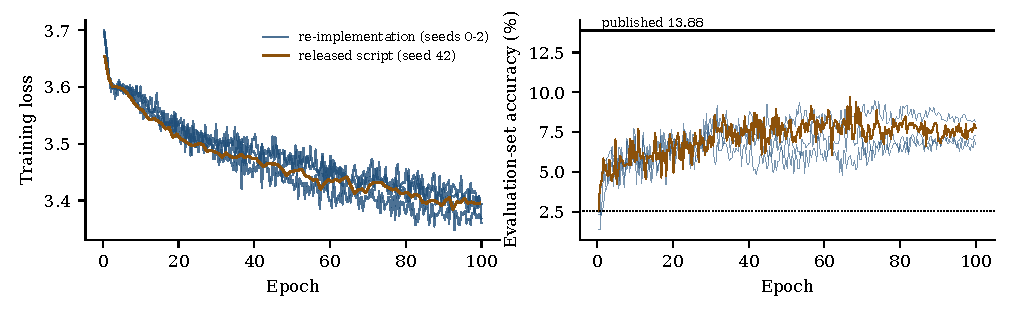
\includegraphics[width=\linewidth]{figures/fig_upstream_check.pdf}
  \caption{\textbf{Re-implementation vs.\ released script}, same configuration (500\,Hz, 100 epochs,
  released split). Left: training loss (ours: mean over each 100-step evaluation interval; released
  script: mean of its printed 10-step losses per epoch). Right: evaluation-set accuracy at every
  evaluation. Ours: seeds 0--2, trained on 4{,}495 trials; released script: seed 42, trained on
  4{,}994. Source: \texttt{results/upstream\_seed42.json} and the 500\,Hz result files.}
  \label{fig:upstream}
\end{figure}

\section{Hyperparameters and compute}
\label{app:hparams}

\begin{table}[ht]
\centering
\small
\begin{tabular}{p{0.24\linewidth}p{0.33\linewidth}p{0.33\linewidth}}
\toprule
 & Reproduction (Table~\ref{tab:repro}) & Split comparison (Table~\ref{tab:splits}) \\
\midrule
Sampling rate & 500\,Hz (1{,}651 samples) & 250\,Hz (825 samples, pairwise mean) \\
Channels & 122 EEG & 122 EEG \\
Epochs & 100 & 30 \\
Optimiser & AdamW, lr $5\times10^{-4}$, wd 0.01 & same \\
Batch size & 16 & 16 \\
Schedule & linear warm-up 10\%, then linear decay & same \\
Evaluation interval & every 100 steps (281 evaluations) & every 100 steps \\
Front end & EEGNet, $F_1{=}8$, $D{=}8$, temporal kernels 20 and 10 & same \\
Encoder & 1 Transformer layer, $d{=}64$, 8 heads, mean pooling & same \\
Dropout & 0.5 (front end), 0.5 (encoder) & same \\
Seeds & 0, 1, 2 & 0, 1, 2 \\
Folds per seed & 1 & interleaved, random: 1; run, session: 3 \\
\bottomrule
\end{tabular}
\caption{Hyperparameters of the two EEG configurations.}
\label{tab:hparams}
\end{table}

All EEG models were trained on one Apple-silicon laptop (PyTorch 2.14.1, MPS backend, float32),
three to four runs sharing the GPU. A 100-epoch run at 500\,Hz took about two hours of training time
under that sharing; the full grid of 39 configurations took about 12 hours, and the released script's
100-epoch run about three hours of training time. The no-EEG classifiers and the drift probe run on CPU in seconds to minutes.

\section{Data checks}
\label{app:data}

\begin{itemize}
\item S1 released imagined-speech epochs: 6{,}243 trials in 45 runs (28--185 per run); every
sentence maps to a category; 39 categories present.
\item In every run, the released sentences are an in-order subsequence of that run's stimulus list
(\path{textdataset/split_data_N.xlsx}); 438 of 6{,}681 presented trials are absent.
\item The BIDS release assigns S1's 45 runs to five sessions of 7, 8, 10, 10 and 10 runs. The paper
describes nine blocks per day; we use the released session labels.
\item Category composition differs between sessions: the total-variation distance between one
session's category distribution and the other four's is 0.39 for session 1 and 0.16--0.23 for the
rest. Session holdout therefore combines a leak-free split with label shift.
\end{itemize}

\section{Reproducing every number}
\label{app:repro}

All code, tests and result files accompany this paper. \texttt{scripts/fetch.sh} downloads
the public data; \texttt{scripts/reproduce\_main\_results.sh} rebuilds the cache, runs the unit
tests, the no-EEG classifiers, the drift probe, every EEG configuration, the released script, and
regenerates all tables and figures from \texttt{results/}. \texttt{paper/README.md} maps each table
and figure to the script and result file that produce it.

\end{document}
